\documentclass{f4_beamer}

\usepackage{iftex}
\ifPDFTeX
   \usepackage[utf8]{inputenc}
   \usepackage[T1]{fontenc}
   \usepackage{lmodern}
\else
   \ifXeTeX
     \usepackage{fontspec}
   \else 
     \usepackage{luatextra}
   \fi
   \defaultfontfeatures{Ligatures=TeX}
\fi

\usepackage{amsmath}
\usepackage{cite}
\usepackage{float}
\usepackage{graphicx}
\graphicspath{{images/}}

\title{Ethereum}
\subtitle{Transaktionen}
\author{Jannes Neemann, Ture Claußen}
\date{\today}

\begin{document}

\section{Gas}
\begin{frame}{Definition}
\begin{itemize}
  \item konzeptioneller Lösungsansatz für das Halteproblem
  \item bemisst einen Ressourcenverbrauch des Weltcomputers
  \item Kosten einer Transaktion: $ \text{\textit{gasPrice}} \times \text{\textit{gasLimit}} $ bzw. $ \text{\textit{gasPrice}} \times \text{\textit{gasUsed}} $ 
\end{itemize}
\end{frame}


\begin{frame}{Intrinsische Kosten $g_0$}
  $$ g_0 \equiv \sum_{i \in T_i, T_d}
  \begin{cases}
    G_{txdatazero} \text{ if } i=0 \\
    G_{txdatanonzero} \text{ otherwise}
  \end{cases}
  +
  \begin{cases}
    G_{txcreate} \text{ if } T_t = \emptyset \\
    0 \text{ otherwise}
  \end{cases}
  +
  G_{transaction}
$$
\end{frame}

\begin{frame}{Intrinsische Kosten von $T_x$}
  \begin{itemize}
  \item $ T_x $ mit $ G_{\text{txdatazero}} \times 4 $ und $ G_{\text{txdatanonzero}} \times 68 \rightarrow $ intrinsische Kosten : 3524 \textit{gas} + 21000 \textit{gas}
  \item Abschätzung: Wie viel Rechenleistung wird zusätzlich gebraucht?
  \end{itemize}
\end{frame}

\begin{frame}{gasPrice von $T_x$}
  \begin{itemize}
  \item Am 20.04.2020 aktzeptieren ungefähr 84\% der letzten 200 Blöcke den Preis von 9GWei
  \end{itemize}
\end{frame}

\begin{frame}{Preis und Latenz}
  \begin{itemize}
  \item Korrelation zwischen gasPrice und Latenz?
  \item Eskalation von Transaktionskosten?
\end{itemize}
\end{frame}

\begin{frame}{Durchsatzfähigkeit}
$$
  T_{max} = \frac{\textit{blockGasLimit}}{\textit{transactionMedianGas}} = \frac{9817880}{80000} = 122.72
$$
\end{frame}

\begin{frame}{blockGasLimit}
um maximal $ \frac{P(H)_{H1}}{1024} $ des alten Limits  $ P(H)_{H1} $ erhöht oder verringert werden darf
\end{frame}


\begin{frame}{Entwicklung gasPrice}
\begin{figure}[h!]
  \centerline{\includegraphics[width=\textwidth, keepaspectratio]{transactions_gasprice_timeseries.png}}
  \caption{gasPrice nach Tag im Monat März \cite{neemann_appendix_nodate}}
  \label{transactions_gasprice_timeseries}
\end{figure}
\end{frame}

\begin{frame}{Preis und Latenz}
  \begin{itemize}
  \item Hohe Auslastung in kleinem Zeitintevall problematisch
  \item ICOs und DOS Angriffe verringern Zuverlässigkeit 
\end{itemize}
\end{frame}

\begin{frame}{}
  \begin{figure}[h!]
    \centerline{\includegraphics[width=\textwidth, keepaspectratio]{blocks_transactions_per_block.png}}
    \caption{Verteilung der Zahl an Transaktionen pro Block (60 konstante Klassen) \cite{neemann_appendix_nodate}}
    \label{blocks_transactions_per_block}
  \end{figure}
  \begin{itemize}
    \item Leere Blöcke lassen sich schneller Veröffentlichen
    \item Wirtschaftliche Interessen gehen vor 
  \end{itemize}
\end{frame}


\begin{frame}{Anreiz und Spieletheorie}
  \begin{itemize}
  \item Warum sollte ich Ressourcen für das System zur Verfügung stellen? $ \rightarrow $Cryptoeconomics
  \item Formalisierung des menschlichen Verhaltens durch Spieletheorie
  \item  \textit{utility payoff} Nützlichkeitsfunktion $ u(x, t) $ möglichst maximieren
\end{itemize}
\end{frame}

\section{Signatur}
\begin{frame}{Bedeutung}
  belegt den Besitz eines Schlüssels, der aktuell die \textit{Authenzität} und die \textit{Integrität} der Nachricht beweisen
\end{frame}

\begin{frame}{Funktion}
  $$
  v, r, s = F_{sig}(F_{keccak256}(m), k)
  $$
  \begin{itemize}
  \item serialisierte Form aller Datenfelder + ChainID
\end{itemize}
\end{frame}

\begin{frame}{Signatur der Transaktion $T_x$}
  \begin{description}
    \item[v:] 26
    \item [r:] dade772f31d20b4ed1c7f63ae035c0cc83fd7b786ca9339eb01763138877a6d4
    \item[s:] 13e16f7a55d261e504e27ea4fecc174a1a46c87d804b9a3917aebde665c1ddb1
  \end{description}
\end{frame}

\section{Propagation}
\begin{frame}{}
  \begin{figure}[h!]
    \centerline{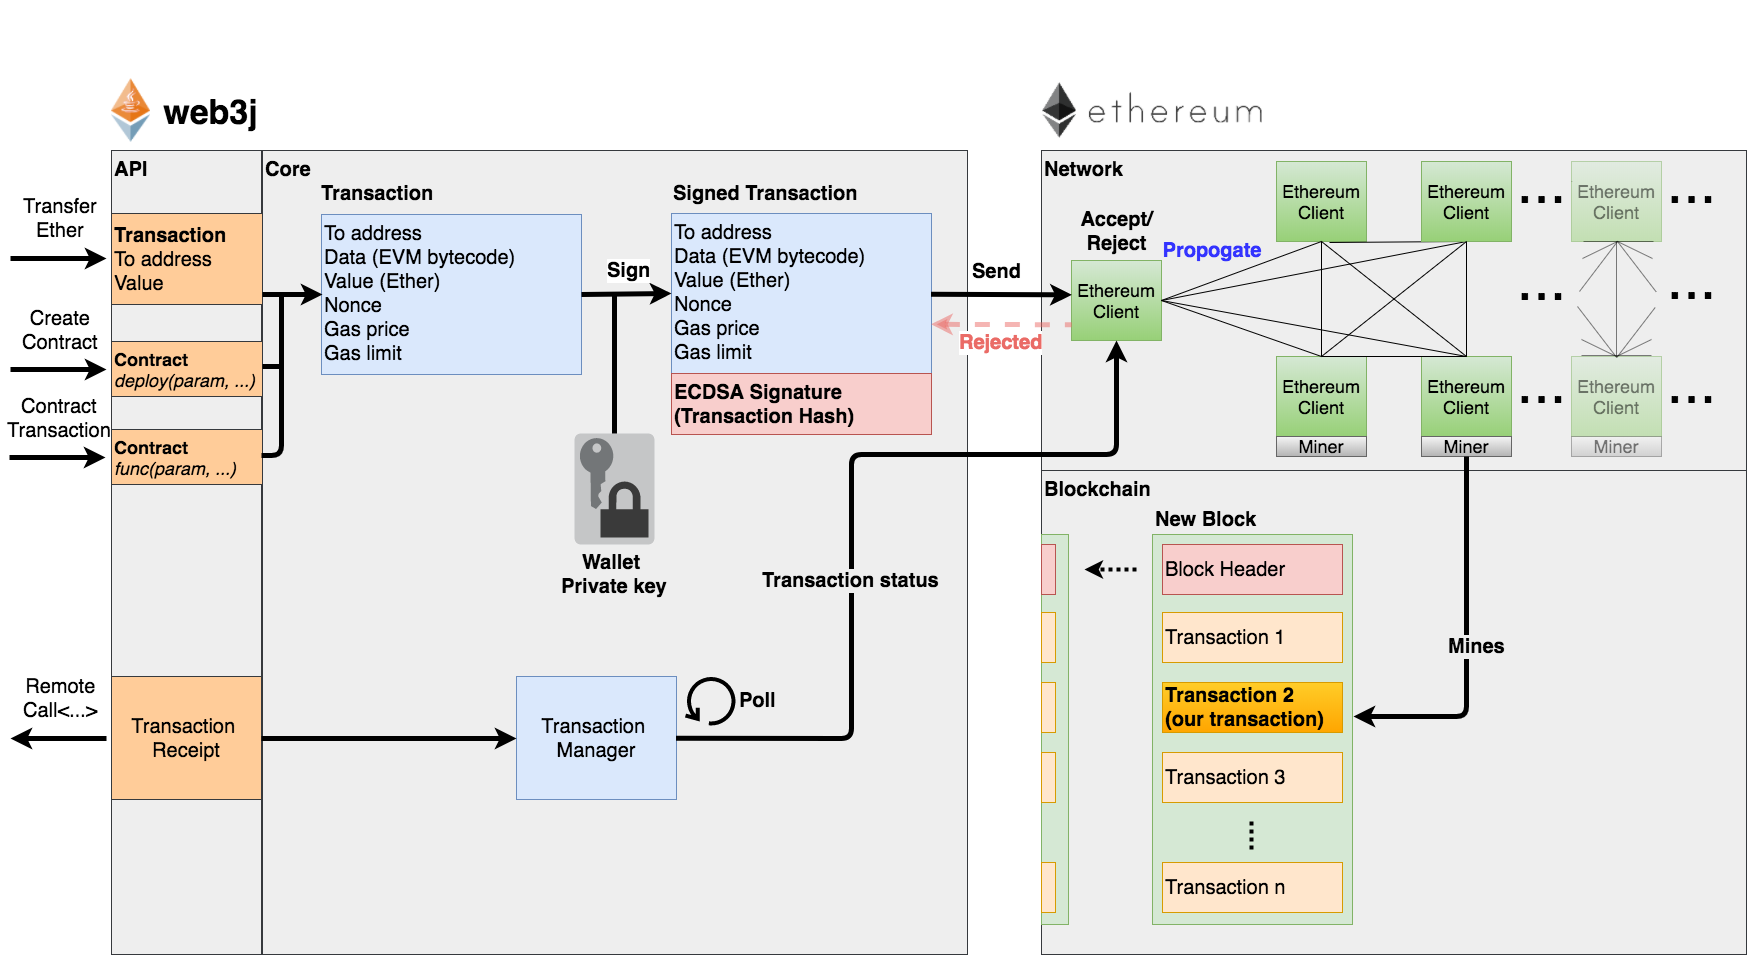
\includegraphics[width=\textwidth, keepaspectratio]{web3j_transaction.png}}
    \caption{Propagation von Client \cite{noauthor_web3j_transactionpng_nodate}}
    \label{blocks_transactions_per_block}
  \end{figure}
  \begin{itemize}
    \item Leere Blöcke lassen sich schneller Veröffentlichen
    \item Wirtschaftliche Interessen gehen vor 
  \end{itemize}
\end{frame}
\begin{frame}{Speicherung}
  \begin{itemize}
    \item Inkludierung im Block
    \item Erstellung eines Receipts \textit{receipt} besteht aus dem Zustand $ R_{\sigma} $ nach der Transaktion, dem kumulierten, verbrauchten Gas nach der Transaktion $ R_u $ und den Logs $ R_l $
    \item \textit{bloom filter} $ R_b $ von den Logs
    \item nach Konsens über Block unveränderlicher Teil der Blockchain
  \end{itemize}
\end{frame}
\section{Ausblick}
\begin{frame}{Ausblick}
  \begin{itemize}
    \item homomorphische Verschlüsselung und Zero-knowledge-proofs
    \item $\rightarrow$ Ethereum 2.0
  \end{itemize}
\end{frame}


\bibliographystyle{splncs04.bst}
\bibliography{paper.bib}
\end{document}
